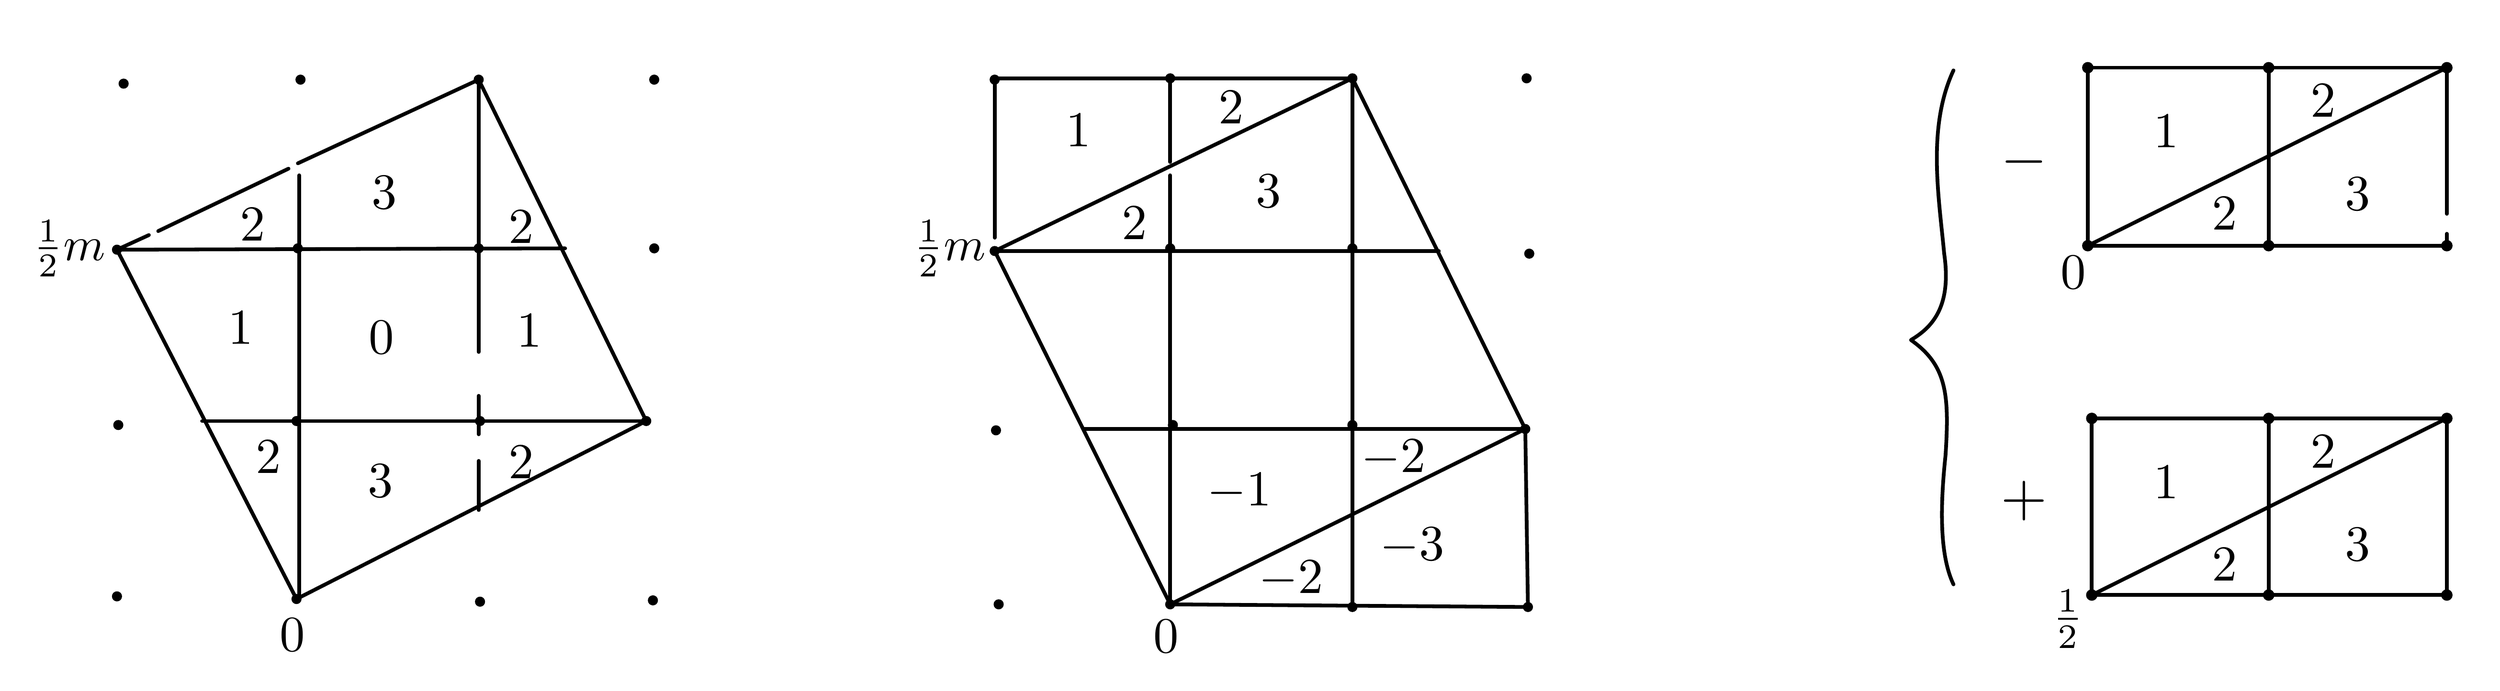
\begin{tikzpicture}[x=1bp,y=-1bp,line cap=round,line join=round]
\path[use as bounding box] (0,0) rectangle (1860,500);
\begin{pgfinterruptboundingbox}
\draw[line width=2.8bp] (78,178) -- (102,167);
\draw[line width=2.8bp] (109,164) -- (207,117);
\draw[line width=2.8bp] (214,113) -- (350,50) -- (476,307) -- (213,441) -- (78,178);
\draw[line width=2.8bp] (215,122) -- (215,441);
\draw[line width=2.8bp] (350,50) -- (350,255);
\draw[line width=2.8bp] (350,288) -- (350,317);
\draw[line width=2.8bp] (350,337) -- (350,374);
\draw[line width=2.8bp] (78,178) -- (415,177);
\draw[line width=2.8bp] (142,307) -- (476,307);
\fill (83,53) circle[radius=3.8bp];
\fill (216,50) circle[radius=3.8bp];
\fill (350,50) circle[radius=3.8bp];
\fill (482,50) circle[radius=3.8bp];
\fill (78,178) circle[radius=3.8bp];
\fill (214,177) circle[radius=3.8bp];
\fill (350,177) circle[radius=3.8bp];
\fill (482,177) circle[radius=3.8bp];
\fill (79,310) circle[radius=3.8bp];
\fill (213,307) circle[radius=3.8bp];
\fill (351,307) circle[radius=3.8bp];
\fill (476,307) circle[radius=3.8bp];
\fill (78,439) circle[radius=3.8bp];
\fill (213,441) circle[radius=3.8bp];
\fill (351,443) circle[radius=3.8bp];
\fill (481,442) circle[radius=3.8bp];
\node[inner sep=0pt,outer sep=0pt,anchor=center] at (180,159) {\scalebox{3.8}{\ensuremath{2}}};
\node[inner sep=0pt,outer sep=0pt,anchor=center] at (279,135) {\scalebox{3.8}{\ensuremath{3}}};
\node[inner sep=0pt,outer sep=0pt,anchor=center] at (382,161) {\scalebox{3.8}{\ensuremath{2}}};
\node[inner sep=0pt,outer sep=0pt,anchor=center] at (171,237) {\scalebox{3.8}{\ensuremath{1}}};
\node[inner sep=0pt,outer sep=0pt,anchor=center] at (277,244) {\scalebox{3.8}{\ensuremath{0}}};
\node[inner sep=0pt,outer sep=0pt,anchor=center] at (388,239) {\scalebox{3.8}{\ensuremath{1}}};
\node[inner sep=0pt,outer sep=0pt,anchor=center] at (192,334) {\scalebox{3.8}{\ensuremath{2}}};
\node[inner sep=0pt,outer sep=0pt,anchor=center] at (276,352) {\scalebox{3.8}{\ensuremath{3}}};
\node[inner sep=0pt,outer sep=0pt,anchor=center] at (382,338) {\scalebox{3.8}{\ensuremath{2}}};
\node[inner sep=0pt,outer sep=0pt,anchor=center] at (42,177) {\scalebox{3.6}{\ensuremath{\frac12 m}}};
\node[inner sep=0pt,outer sep=0pt,anchor=center] at (210,468) {\scalebox{3.8}{\ensuremath{0}}};
\draw[line width=2.8bp] (738,179) -- (1007,49) -- (1137,313) -- (870,445) -- cycle;
\draw[line width=2.8bp] (738,169) -- (738,49) -- (1007,49);
\draw[line width=2.8bp] (870,445) -- (1139,447) -- (1137,313);
\draw[line width=2.8bp] (870,49) -- (870,112);
\draw[line width=2.8bp] (870,122) -- (870,445);
\draw[line width=2.8bp] (1007,49) -- (1007,447);
\draw[line width=2.8bp] (738,179) -- (1072,179);
\draw[line width=2.8bp] (805,313) -- (1137,313);
\fill (738,50) circle[radius=3.8bp];
\fill (870,49) circle[radius=3.8bp];
\fill (1007,49) circle[radius=3.8bp];
\fill (1138,49) circle[radius=3.8bp];
\fill (738,179) circle[radius=3.8bp];
\fill (870,177) circle[radius=3.8bp];
\fill (1007,177) circle[radius=3.8bp];
\fill (1140,181) circle[radius=3.8bp];
\fill (739,314) circle[radius=3.8bp];
\fill (872,310) circle[radius=3.8bp];
\fill (1007,310) circle[radius=3.8bp];
\fill (1137,313) circle[radius=3.8bp];
\fill (741,445) circle[radius=3.8bp];
\fill (870,445) circle[radius=3.8bp];
\fill (1007,447) circle[radius=3.8bp];
\fill (1139,447) circle[radius=3.8bp];
\node[inner sep=0pt,outer sep=0pt,anchor=center] at (801,88) {\scalebox{3.8}{\ensuremath{1}}};
\node[inner sep=0pt,outer sep=0pt,anchor=center] at (843,158) {\scalebox{3.8}{\ensuremath{2}}};
\node[inner sep=0pt,outer sep=0pt,anchor=center] at (916,71) {\scalebox{3.8}{\ensuremath{2}}};
\node[inner sep=0pt,outer sep=0pt,anchor=center] at (944,134) {\scalebox{3.8}{\ensuremath{3}}};
\node[inner sep=0pt,outer sep=0pt,anchor=center] at (922,360) {\scalebox{3.8}{\ensuremath{-1}}};
\node[inner sep=0pt,outer sep=0pt,anchor=center] at (961,426) {\scalebox{3.8}{\ensuremath{-2}}};
\node[inner sep=0pt,outer sep=0pt,anchor=center] at (1038,335) {\scalebox{3.8}{\ensuremath{-2}}};
\node[inner sep=0pt,outer sep=0pt,anchor=center] at (1052,401) {\scalebox{3.8}{\ensuremath{-3}}};
\node[inner sep=0pt,outer sep=0pt,anchor=center] at (704,177) {\scalebox{3.6}{\ensuremath{\frac12 m}}};
\node[inner sep=0pt,outer sep=0pt,anchor=center] at (867,469) {\scalebox{3.8}{\ensuremath{0}}};
\draw[line width=2.8bp] (1459,43) .. controls (1439,86) and (1448,138) .. (1452,181) .. controls (1458,222) and (1442,237) .. (1427,246) .. controls (1454,265) and (1456,287) .. (1453,333) .. controls (1448,380) and (1450,411) .. (1459,430);
\draw[line width=2.8bp] (1830,151) -- (1830,41) -- (1560,41) -- (1560,175) -- (1830,175) -- (1830,166);
\draw[line width=2.8bp] (1696,41) -- (1696,175);
\draw[line width=2.8bp] (1560,175) -- (1830,41);
\fill (1560,41) circle[radius=4.3bp];
\fill (1696,41) circle[radius=4.3bp];
\fill (1830,41) circle[radius=4.3bp];
\fill (1560,175) circle[radius=4.3bp];
\fill (1696,175) circle[radius=4.3bp];
\fill (1830,175) circle[radius=4.3bp];
\node[inner sep=0pt,outer sep=0pt,anchor=center] at (1619,89) {\scalebox{3.8}{\ensuremath{1}}};
\node[inner sep=0pt,outer sep=0pt,anchor=center] at (1663,151) {\scalebox{3.8}{\ensuremath{2}}};
\node[inner sep=0pt,outer sep=0pt,anchor=center] at (1737,66) {\scalebox{3.8}{\ensuremath{2}}};
\node[inner sep=0pt,outer sep=0pt,anchor=center] at (1763,136) {\scalebox{3.8}{\ensuremath{3}}};
\draw[line width=2.8bp] (1563,305) -- (1830,305) -- (1830,438) -- (1563,438) -- cycle;
\draw[line width=2.8bp] (1696,305) -- (1696,438);
\draw[line width=2.8bp] (1563,438) -- (1830,305);
\fill (1563,305) circle[radius=4.3bp];
\fill (1696,305) circle[radius=4.3bp];
\fill (1830,305) circle[radius=4.3bp];
\fill (1563,438) circle[radius=4.3bp];
\fill (1696,438) circle[radius=4.3bp];
\fill (1830,438) circle[radius=4.3bp];
\node[inner sep=0pt,outer sep=0pt,anchor=center] at (1619,353) {\scalebox{3.8}{\ensuremath{1}}};
\node[inner sep=0pt,outer sep=0pt,anchor=center] at (1663,415) {\scalebox{3.8}{\ensuremath{2}}};
\node[inner sep=0pt,outer sep=0pt,anchor=center] at (1737,330) {\scalebox{3.8}{\ensuremath{2}}};
\node[inner sep=0pt,outer sep=0pt,anchor=center] at (1763,400) {\scalebox{3.8}{\ensuremath{3}}};
\node[inner sep=0pt,outer sep=0pt,anchor=center] at (1512,112) {\scalebox{4.5}{\ensuremath{-}}};
\node[inner sep=0pt,outer sep=0pt,anchor=center] at (1512,367) {\scalebox{4.5}{\ensuremath{+}}};
\node[inner sep=0pt,outer sep=0pt,anchor=center] at (1549,195) {\scalebox{3.8}{\ensuremath{0}}};
\node[inner sep=0pt,outer sep=0pt,anchor=center] at (1545,456) {\scalebox{3.7}{\ensuremath{\frac12}}};
\end{pgfinterruptboundingbox}
\end{tikzpicture}
